%!TEX root = ../thesis.tex

\chapter{Technologies}\label{chapter:technologies}

	To fully understand the project and the choices behind it, is worth taking a look at some backgrounds technology which can be useful to know before proceeding further into this thesis.
	In this chapter we describe DTNs, the notion of peer-to-peer and overlay networks.

	

	\section{Radio technologies}\label{sec:section_two}
	
		\begin{figure}
			\centering
			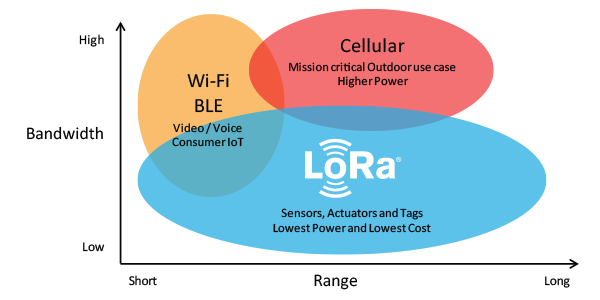
\includegraphics[width=\textwidth]{resources/img/LoRa_Why_Range}
			\caption{}
		\end{figure}
	
		\subsection{LoRa}
		
		https://lora-alliance.org/
		
		https://www.semtech.com/lora
		
		\subsection{LoRaWAN}
		
		\subsection{Bluetooth}		
		
		\subsection{WiFi}
		
		IEEE 802.11, better known in the public as WiFi, short for wireless fidelity
	
		\subsection{LTE}
	
	\section{LoRa and LoRaWAN}
	
	\section{Hardware (Microcontrollers)}
	
	\subsection{Arduino}
	
	\subsection{Raspberry Pi}
	
	\subsection{Pycom}